\documentclass[11pt]{article}
\pdfinfoomitdate=1\pdftrailerid{}
\usepackage[letterpaper,margin=.7in,headheight=15pt,headsep=18pt,footskip=24pt]{geometry}
\usepackage[T1]{fontenc}\usepackage{lmodern,amsmath,amssymb,array,booktabs,fancyhdr,hyperref,tikz}
\renewcommand{\familydefault}{\sfdefault}\setlength{\parindent}{0pt}\setlength{\parskip}{6pt}
\pagestyle{fancy}\fancyhf{}\fancyhead[L]{\small Week NN / Breaking and drawing games / Facilitator guide}
\fancyfoot[L]{\scriptsize Bellingham Math Circle / Week NN / NN-FAC-v1}\fancyfoot[R]{\thepage}
\hypersetup{hidelinks}
\newcommand{\head}[1]{\par\textbf{\large #1}\par}
\newcommand{\sub}[1]{\par\textbf{#1}\par}
\newcommand{\by}{\,$\times$\,}
\begin{document}
\head{Mathematical overview: a count that every move changes}
All four games use the normal rule: whoever makes the last move wins. If every game on a board lasts the same number of moves $N$, the first player wins when $N$ is odd and the second when $N$ is even, whatever anyone chooses. Three games here have that property because a count changes by the same amount every move and the game cannot stop until the count reaches a value fixed at the start: pieces of the bar (up one per break), tokens in 2-Sprigs (down two per line) and, in Brussels Sprouts, regions minus separate pieces of the drawing (up one per move). Sprouts has a count that drops by one every move, but the game can stop before it runs out.

\textbf{Breaking bars: every order takes $mn-1$ breaks.} A break splits one piece along one full grid line into two pieces. Each break turns one piece into two, so the number of pieces rises by exactly one, from $1$ to $mn$. More generally, pieces with $S$ squares in all, $P$ pieces at the start, take $S-P$ breaks. So in ``last break wins'' the first player wins exactly when $mn$ is even, that is, when a side is even; the fewest and the most breaks are the same number. \emph{Limit:} one piece per break is essential. If pieces could be stacked and cut together, a 3\by4 bar would need only 4 cuts (no fewer, since a cut at most doubles the number of pieces: $1,2,4,8<12$).

\textbf{2-Sprigs: $n$ dots, exactly $n$ moves.} Each dot has two tokens; each end of a line uses one, so a loop needs two; a line may not cross itself or another line, or touch another dot. \emph{At most $n$ moves:} there are $2n$ tokens and every move uses two. \emph{The game cannot stop while a token remains:} since no dot has more than two line ends, the drawing consists of closed loops, open chains and untouched dots. An untouched dot can always draw a small loop. A dot with one token is the end of a chain whose other end also has one token; a chain encloses nothing, so its two ends border the same region and can be joined. Hence every game uses every token, and the first player wins exactly when $n$ is odd. \emph{Limits:} the two clarifications in the printed rules carry the theorem. A loop at a one-token dot, or a line that crosses itself and shuts a dot in, makes lengths vary and changes winners. With three tokens per dot (3-Sprigs) the length varies: 4 dots last 5 or 6 moves.

\textbf{Brussels Sprouts: $n$ crosses, exactly $5n-2$ moves} (3, 8, 13, 48 for 1, 2, 3, 10 crosses). A move joins two free arms by a line and draws a short bar across it, a new cross with one new free arm on each side. (1) The number of free arms never changes: each move uses two and makes two, so there are always $4n$. (2) Each separate piece of a region's edge always keeps a free arm pointing into that region: when a line cuts a region in two, its bar sends a new arm into each half. (3) At the end no region holds two free arms, or they could be joined. So a finished game has exactly $4n$ regions. A finished region holds only one free arm, so its edge is in one piece, and therefore the whole drawing is in one piece. (4) Regions minus separate pieces of the drawing starts at $1-n$ and rises by exactly one every move: a line between two pieces joins them into one, and a line within one piece cuts a region in two. At the end it is $4n-1$, so there are $(4n-1)-(1-n)=5n-2$ moves. This is Euler's formula built one move at a time; Grades 4--5 Problem 11 uses the formula itself. Counting crosses as dots and each piece of line from one cross to the next as a line, after $m$ moves there are $n+m$ dots and $2m$ lines, and dots $-$ lines $+$ regions $=2$ for a drawing in one piece gives $(n+m)-2m+4n=2$, so $m=5n-2$.

\textbf{Sprouts: a bound, not a fixed length.} Each spot has three tokens, and each move puts a new spot with one token on its line. A move removes two tokens and adds one, so the total drops by exactly one; the newest spot always keeps its token, so $n$ spots last at most $3n-1$ moves. Cooperative play reaches this by keeping every spot with a token on the edge of one region: join two such spots that are next to each other along that edge, or loop a spot without enclosing any other spot that has a token. Merely never shutting a spot in alone is not enough: two groups of spots with tokens can be cut off from each other, and each group then keeps a token. Every game lasts at least $2n$ moves (Wikipedia), and loop-then-join play (see the Grades 4--5 Problem 7 solution) reaches $2n$. So 2 spots last 4 or 5 moves, 3 spots 6, 7 or 8, and choices decide the winner. With best play the second player wins with 1 or 2 spots and the first with 3 (our exhaustive check), 4 or 5; the second with 6 or 7 (published analyses). Applegate, Jacobson and Sleator (1991) conjectured that the first player wins exactly when $n$ leaves remainder 3, 4 or 5 on division by 6.

\textbf{What children discover, and how sure they can be.} \emph{Experiments:} repeated games, recording the winner and the number of moves. \emph{Conjectures:} ``the 2nd player always wins the 3\by3 bar'', ``as many lines as dots'', ``five more moves for each cross''. \emph{Explanations:} one more piece per break; tokens used two at a time with no early stop; one free arm per region with Euler's formula; the token bound in Sprouts. Repeated games are evidence, not proof; a game that breaks a pattern refutes it only once it is checked for an illegal move.

\textbf{Map of the bands.} \emph{K--1} (rules read aloud, counting to 12): count breaks with a counter in a cup and find the count never changes; play ``last break wins'' and 2-Sprigs on 2 to 6 dots and notice that the same seat (1st or 2nd) wins a given bar or board every time; Problem 8 runs the count backwards. \emph{Grades 2--3} (short rules, counting to about 40): predict winners of bars and Sprigs boards and explain with ``one more piece each break'' and ``as many lines as dots''; then Sprouts, where choices change the winner and tokens bound the length. \emph{Grades 4--5} (reads the rule paragraphs; multiplies 8\by13 and 25\by40): explain the counts and the even-side rule, prove 2-Sprigs cannot stop early, bound Sprouts (29 moves for 10 spots), predict Brussels Sprouts, and meet Euler's formula as the reason for $5n-2$.

\head{Preparation, launch and pacing}
\textbf{Status.} Prepared for organizer review; unpiloted. Not physically tried: children cutting card bars along 25\,mm lines (time, card weight and scissor skill, especially K--1, whose first route needs about 54 cuts per pair), trimming the bar sheets, cube slabs breaking cleanly along a line, counters fitting beside spots once new spots appear (tightest: the 3-spot Sprouts boards, Grades 2--3 Problem 8 and Grades 4--5 Problem 7, spots 69\,mm apart), partners removing tokens reliably, and all timings.

\textbf{Materials file.} \texttt{materials.pdf} (3 pages, beside the packets) prints what no packet supplies. Page~1, \emph{Bars, sheet 1}: two 3~by~4, two 3~by~3, a 2~by~4, a 2~by~3 and a 1~by~6 bar. Page~2, \emph{Bars, sheet 2}: a 3~by~4, a 3~by~3, two 2~by~4, a 2~by~3, two 2~by~2 and the 2~by~5 launch bar. Squares are 25\,mm; the adult trims along the heavy outlines and children break along the thin grid lines. The bars drawn in the packets are smaller pictures and are not cut, and the bars children decide about without breaking (Problem 3 in Grades 2--3 and 4--5) are deliberately not supplied. Page~3, \emph{2-spot Sprouts boards}: two boards 186~by~102\,mm with spots 90\,mm apart, for Grades 4--5 Problem 6 in place of the cramped boards (spots 44\,mm apart) on that page.

\textbf{Per pair.} One \emph{Bars, sheet 1} plus a 2~by~4 and a 2~by~2 from the table's \emph{Bars, sheet 2}: nine bars, 74 squares, for K--1 Problems 1--3 or Grades 2--3 Problems 1--2; the second 3~by~4 is for a second try at Problem 2. The rest of the table's sheet 2 (a 3~by~4, a 3~by~3, a 2~by~3 and the 2~by~5) is a spare pool in the middle of the table, for a recount and for checking K--1 Problem 8. The Grades 4--5 trio gets a whole sheet 1 and sheet 2, 15 bars: Problems 1--2 use five, and the spare 3~by~3 and 2~by~4 give the referee a game or, with a 2~by~3, test the last question of Problem 3 after deciding. Bars are used up when cut. \emph{Child scissors,} one per child. \emph{Fifteen counters} no wider than about 12\,mm (dried beans work) for tokens, kept in a row under each dot as in the rule pictures; K--1 also needs a cup. \emph{Pencils;} Grades 4--5 also a small whiteboard and marker (Problem 9).

\textbf{Print and prepare.} The organizer prepares ahead, so the table adults need only read their band's pages and this guide. One packet per child, single-sided US Letter at 100\%: K--1 7 pages, Grades 2--3 7, Grades 4--5 9 (83 pages for the current eleven children). A pair plays on one child's boards and uses the partner's packet for further games; nothing in the packets is cut. From \texttt{materials.pdf}, single-sided at 100\% on light card stock: page~1 once per pair or trio and page~2 once per table of two pairs, so for the current tables (two K--1 pairs, two 2--3 pairs, one 4--5 trio) 5 copies of page~1 and 3 of page~2, 8 card sheets and 59 bars; page~3 once on plain paper for the 4--5 table. Trim each card sheet along the heavy outlines, full-width strips first, then bars: 11 cuts for page~1 and 12 for page~2, 91 in all. Put each pair's nine bars in an envelope with its counters, and each table's four spare bars in another. Estimate 35 minutes the first time: 10 to print, 15--20 to trim with a paper trimmer (two copies of one page can go through together; scissors take longer), 5 to fill envelopes. This estimate needs a rehearsal. For a K--1 return visit with Problem 8, print one more page~2. \emph{Lower-preparation route,} at K--1 or at every table: flat slabs of interlocking cubes instead of card bars, 12 cubes per pair (enough for one 3~by~4 slab at a time), rebuilt after each game; with no card to print or trim, preparation is about 20 minutes.

\textbf{Staffing.} One adult per table. At K--1 the adult reads rules aloud and may hold a bar steady; the child chooses each break, and the partner drops a counter in the cup for each break and takes away tokens. If cutting is slow, the child points to the line and the partner or adult cuts; the child still chooses every break. If even that drags, switch the table to cube slabs. At every table the partner (at Grades 4--5 the third child as referee, rotating) checks each break or line. Adults do not announce winners before a game or name the rule. Writing down numbers a child says is ordinary support; an adult choosing breaks or lines means the bar or board is too big. Give the player who starts a spare counter to hold, so the pair remembers who went first.

\textbf{Whole-group launch, five minutes.} Gather the children round one table and pass round a 2~by~5 bar (from page~2 of the materials; no problem uses it) and a few counters. Cut the bar once along a full line into a 2~by~2 and a 2~by~3, the picture at the top of each packet's page~1, and have a child drop a counter in a cup. Cut one piece once more. Show what is not allowed: stacking two pieces and cutting both, stopping partway, cutting round a corner. Stop there without finishing or counting the whole bar. Then draw seven dots on a sheet of paper (no page uses seven) and put two counters beside each. Two children play: one draws a line between two dots, and the other, as partner, takes away one counter at each end; then the second child loops a fresh dot, and the first takes away both of its counters. Show that a loop at a dot with one counter left is not allowed. Stop after two moves. Show the record: circle 1st or 2nd for the seat of the player who made the last move, not a name. The figure is the adult's reference; a whiteboard with magnets as tokens also works.

\begin{center}
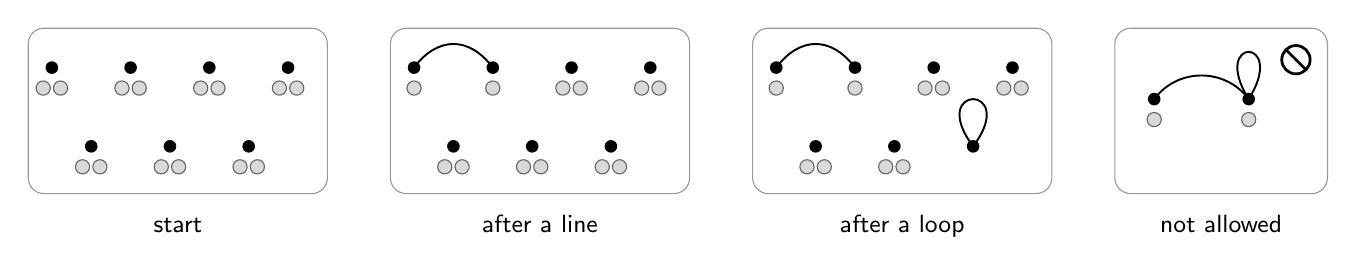
\begin{tikzpicture}[x=1mm,y=1mm,font=\small]
\newcommand{\board}[2]{% offset, state 0/1/2
  \begin{scope}[shift={(#1,0)}]
    \draw[black!40,rounded corners=2mm] (-3,-4) rectangle (35,17);
    \foreach \x/\y in {0/12,10/12,20/12,30/12,5/2,15/2,25/2}{\fill (\x,\y) circle (0.8);}
  \end{scope}}
\newcommand{\tok}[2]{\draw[black!60,fill=black!15] (#1,#2) circle (0.9);}
% panel 1: start
\board{0}{0}
\foreach \x/\y in {0/12,10/12,20/12,30/12,5/2,15/2,25/2}{\tok{\x-1.1}{\y-2.6}\tok{\x+1.1}{\y-2.6}}
\node[anchor=base] at (16,-9) {start};
% panel 2: after a line between two dots
\begin{scope}[shift={(46,0)}]
\board{0}{0}
\draw[line width=.7pt] (0,12) .. controls (3,16) and (7,16) .. (10,12);
\tok{0}{9.4}\tok{10}{9.4}
\foreach \x/\y in {20/12,30/12,5/2,15/2,25/2}{\tok{\x-1.1}{\y-2.6}\tok{\x+1.1}{\y-2.6}}
\node[anchor=base] at (16,-9) {after a line};
\end{scope}
% panel 3: after a loop
\begin{scope}[shift={(92,0)}]
\board{0}{0}
\draw[line width=.7pt] (0,12) .. controls (3,16) and (7,16) .. (10,12);
\draw[line width=.7pt] (25,2) .. controls (19,10) and (31,10) .. (25,2);
\tok{0}{9.4}\tok{10}{9.4}
\foreach \x/\y in {20/12,30/12,5/2,15/2}{\tok{\x-1.1}{\y-2.6}\tok{\x+1.1}{\y-2.6}}
\node[anchor=base] at (16,-9) {after a loop};
\end{scope}
% panel 4: not allowed
\begin{scope}[shift={(138,0)}]
\draw[black!40,rounded corners=2mm] (-3,-4) rectangle (24,17);
\fill (2,8) circle (0.8); \fill (14,8) circle (0.8);
\draw[line width=.7pt] (2,8) .. controls (5,12) and (11,12) .. (14,8);
\draw[line width=.7pt] (14,8) .. controls (9,16) and (19,16) .. (14,8);
\tok{2}{5.4}\tok{14}{5.4}
\draw[line width=1pt] (20,13) circle (1.8); \draw[line width=1pt] (18.7,14.3) -- (21.3,11.7);
\node[anchor=base] at (10.5,-9) {not allowed};
\end{scope}
\end{tikzpicture}
\end{center}

\textbf{At the tables.} Before Sprouts (Grades 2--3 Problem 6, Grades 4--5 Problem 6) and Brussels Sprouts (Grades 4--5 Problem 9), the table adult plays one move with a child on a scrap board of four spots or four crosses, which no page uses: in Sprouts the drawer adds the new spot and gives it one token; in Brussels Sprouts the bar crosses the line so one new arm points to each side.

\textbf{A first hour.} After five minutes of running around and the launch, tables have 35--40 minutes. \emph{K--1:} Problems 1--3 (about 25 minutes of breaking), then Problem 4. \emph{Grades 2--3:} Problems 1--4, then Problem 6, so that the first hour reaches the contrast with Sprouts, which is the theme's point; a quick table does Problem 5 before Problem 6. \emph{Grades 4--5:} Problems 1--5. In the last minutes ask each table one question to share: K--1 ``Who won on the square bar?'', Grades 2--3 ``Does Sprouts with 2 spots always last the same number of moves?'', Grades 4--5 ``Why can't 2-Sprigs stop early?''.

\textbf{Return visits.} \emph{K--1:} one 2-Sprigs game to recall the tokens, then Problems 5--8. \emph{Grades 2--3:} Problem 5 if it was skipped (decide first, then 10 and 25 dots), then Sprouts again, Problems 7--8. \emph{Grades 4--5:} Problems 6--9 (Sprouts and the first Brussels games), then Problems 10--11, keeping the finished Problem 9 drawings. Readiness-dependent extensions are with each band's solutions. Finishing every page is not the goal.

\head{Grades K--1 (7 pages): breaks, last break wins, 2-Sprigs}
\emph{Key in plain words for the adult:} a bar always takes one break fewer than it has squares, in any order, so on a given bar the same seat wins every game. In 2-Sprigs every game uses up every token, two per line, so there are as many lines as dots. Let children find ``it's the same every time''; the reasons are for the adult, and for a child who asks.

\sub{Problem 1, page 1: break three bars}
Bars from the pair's envelope (materials pages 1--2). 3 breaks for the 2\by2, 5 for the 2\by3, 5 for the 1\by6. Children may notice that two different-looking bars take the same number. If two counts for the same bar differ, look for a missed counter or two pieces cut together, and break a bar from the table's spare pool with the adult watching. Prompt before the second bar: ``How many counters do you think will go in the cup?''

\sub{Problem 2, page 2: as few breaks as you can}
11 breaks, whatever the order; nobody can do it with fewer, or with more. The discovery is the table comparison: pairs that broke differently all get 11. A child's explanation: ``every break made one more piece; we started with one piece and ended with 12 squares.'' Hint, for a child sure a clever order saves breaks: ``Which break would you skip? Try it on your second 3~by~4.''

\sub{Problem 3, page 2: last break wins}
3\by3: 8 breaks, the 2nd player wins every game. 2\by4: 7 breaks, the 1st player wins every game. Because the starting player changes, each child wins once on each bar, so the pattern shows in the circles, not in the names. Hint: ``Look at your circles for the square bar. What do you notice?'' Extension: ``Which bar would you want to go first on?''

\sub{Problem 4, page 3: first 2-Sprigs games}
2 dots: 2 lines, 2nd player wins. 3 dots: 3 lines, 1st player wins. Every game. Usual slips: a loop at a dot with one token (third rule picture), a line through a dot (fifth picture), tokens not taken away. A game is over when no line can be drawn. Hint: ``Are there any tokens left? Can anyone still draw?''

\sub{Problem 5, page 4: count the lines}
Every 4-dot game has 4 lines and the 2nd player wins. The tokens check the count: 8 tokens, two per line. Hint: ``How many tokens did each line take away?''

\sub{Problem 6, page 5: can the 2nd player win with 5 dots?}
No. Every game has 5 lines, and the 1st player draws lines 1, 3 and 5. ``It never happened in our four games'' is an honest experimental answer; ``10 tokens, two for each line'' is the explanation a K--1 child can give. Why the game cannot stop with tokens left is in the overview and need not come up. If a pair says the 2nd player won, replay that game together and look for an illegal line.

\sub{Problem 7, page 6: guess, then play}
6 dots: 6 lines, the 2nd player wins both games. Any guess is fine; the goal is a reason such as ``like the 4 dots'' or ``six lines, so the 2nd player draws the last one''.

\sub{Problem 8, page 7: how many breaks made each group?}
2, 4 and 6. The groups have 3, 5 and 7 pieces (for example from a 2\by3, a 3\by3 and a 3\by4 bar), and each break makes one more piece. The tempting answers 5, 8 and 11 are what breaking the whole bar into single squares takes. Check by breaking the spare pool's 2~by~3, 3~by~3 and 3~by~4 (materials page 2) into the same pieces with the cup. For the third group: break off the 1\by4 row, then a 2\by1 column from the 2\by4 left over, split the 2\by3 into two 1\by3 strips, and cut those into a 1\by2 and four single squares with three more breaks, 6 in all. Hint: ``How many pieces were there before the first break? After one break?''

\head{Grades 2--3 (7 pages): predict, explain, then Sprouts}
\sub{Problem 1, page 1: last break wins}
Bars from the pair's envelope (materials pages 1--2). 3\by3: 8 breaks, the 2nd player wins both games. 2\by4: 7 breaks, the 1st player wins both. No: every way of breaking a bar takes the same number of breaks, so the loser cannot change the result. Children first answer from evidence (``we tried different ways''); the explanation often arrives during Problem 2 or 3. Follow-up: ``How do you know a cleverer order would not change it?''

\sub{Problem 2, page 1: fewest breaks}
11, 5 and 3. The fewest is also the most. A child hunting for a shortcut, for example three strips first, can try it on the pair's second 3~by~4 and still counts 11. If a pair reports fewer, look for stacked pieces.

\sub{Problem 3, page 2: decide without breaking}
4\by5: 19 breaks, 1st. 3\by5: 14, 2nd. 5\by5: 24, 2nd. 1\by9: 8, 2nd. 6\by6: 35, 1st. Explanation: breaks $=$ squares $-1$, because every break makes one more piece, and an odd number of breaks means the 1st player makes the last. ``Odd by odd is a 2nd-player bar'' is a correct rule; ask for its reason. Hint: ``How many squares did the 3\by3 have, and how many breaks did it take?'' Extension: which bars would you want to go second on? (Both sides odd.)

\sub{Problem 4, page 3: 2-Sprigs on 3 and 4 dots}
3 dots: 3 moves, 1st player. 4 dots: 4 moves, 2nd player. Every game. The moves record is the evidence Problem 5 needs. A different count means an illegal move (a loop at a one-token dot, a line through a dot or across itself) or a token not taken away.

\sub{Problem 5, page 4: decide first; 10 and 25 dots}
5 dots: 1st (5 moves). 6 dots: 2nd (6 moves). 10 dots: 2nd. 25 dots: 1st. A full Grades 2--3 explanation: ``Each dot has 2 tokens and each line uses 2, so if the game uses all the tokens there are as many lines as dots; an odd number of dots means the 1st player draws the last line.'' At this level ``the game uses all the tokens'' rests on experiment; the follow-up ``Could a game stop while a dot still has a token?'' is Grades 4--5 Problem 5. Hint: ``Look at your moves on page 3. What do you notice?''

\sub{Problem 6, page 5: Sprouts with 1 and 2 spots}
1 spot: always 2 moves, so the 2nd player wins. The first move must be a loop; the old spot and the new spot then have one token each and are joined; the third spot is alone with one token. 2 spots: 4 or 5 moves, so either player can win. Watch for a forgotten new spot or its token, which shortens a game.

\sub{Problem 7, page 6: longest and shortest 2-spot games}
Longest 5, shortest 4; yes, the choices change the winner (5 moves, 1st player; 4 moves, 2nd). With spots A and B and the new spots lettered in order, five moves: A--B (C); A--B again, making a ring A--C--B--D (D); inside the ring A--C (E); still inside, in the part with E, B--D (F); E--F (G), and only G keeps a token. Four moves: A loops (C); inside the loop A--C (D), which shuts D in alone; B loops (E); B--E (F). Hints: for the short game, ``Can you leave a spot with a token where no other spot can reach it?''; for the long game, ``Can every spot that still has a token reach the others?''

\sub{Problem 8, page 7: longest game with 3 spots}
8. There are 9 tokens at the start; each move takes away 2 and adds 1, so after every move there is one token fewer; the newest spot always keeps its token, so at least one is left. An 8-move game, with spots A, B, C and the new spots lettered in order: A--B (D); B--C (E); A--C (F), which closes a ring; then, all on one side of the ring, A--D (G), G--B (H), H--E (I), I--C (J), J--F (K); only K keeps a token. A full answer has both a game of 8 and the reason there is no game of 9. Hint: ``How many tokens are on the board at the start? After one move? After two?'' Extension: 10 spots (29; Grades 4--5 Problem 8).

\head{Grades 4--5 (9 pages): proofs, bounds and Euler's formula}
\sub{Problems 1--2, page 1: last break wins; fewest and most}
Bars as in Grades 2--3, with a spare 3~by~3, 2~by~4 and 3~by~4 for the referee. Problem 1 as in Grades 2--3. Problem 2: fewest $=$ most $=11$, since the pieces go from 1 to 12, one per break. Extension, a rule change: if pieces could be stacked, 4 cuts would do and 3 never could, since a cut at most doubles the number of pieces. This is why the rules say never stack.

\sub{Problem 3, page 2: a rule for any bar}
7\by9: 63 squares, 62 breaks, 2nd. 8\by13: 104 squares, 103 breaks, 1st. 25\by40: 1000 squares, 999 breaks, 1st. Rule: the 1st player wins exactly when the number of squares is even, that is, when a side is even, because there are always squares $-1$ breaks. Starting with a 2\by3 and a 2\by4: 14 squares in 2 pieces, so 12 breaks, and the 2nd player wins. The slip ``$14-1=13$'' misses that the game starts with two pieces; ask ``How many pieces are on the table before the first break?''

\sub{Problem 4, page 3: 2-Sprigs on 3 and 4 dots}
As Grades 2--3 Problem 4: 3 moves and the 1st player; 4 moves and the 2nd.

\sub{Problem 5, page 4: can a game stop with a token left?}
No, so with $n$ dots every game lasts $n$ moves and the 1st player wins exactly when $n$ is odd (proof in the overview). Attempts that fail: a loop from another dot drawn round a one-token dot cannot cross that dot's chain, so it surrounds the whole chain and both ends stay together; two untouched dots in different regions can each still loop. A child's proof: ``A dot with one token is the end of a chain. Follow the chain; its other end has one token too, and nothing can get between them, so they can be joined.'' If a child succeeds, look for a line that crosses itself or a loop at a one-token dot, both forbidden. Hint: ``What do you know about a dot that has only one token left?'' Extension: 3-Sprigs, with three tokens per dot: 4 dots can last 5 or 6 moves, so the winner is no longer fixed.

\sub{Problem 6, page 5: Sprouts, 2 spots}
Play on the two boards of materials page 3 (spots 90\,mm apart, with room for counters and new spots) and write the moves on the page. Longest 5, shortest 4; yes, choices change the winner. Example games are under Grades 2--3 Problem 7. Background: with best play the 2nd player wins with 2 spots.

\sub{Problem 7, page 6: Sprouts, 3 spots}
Longest 8, shortest 6 (7 also occurs). Six: for each spot in turn, loop, then join the spot to the loop's new spot inside the loop, which shuts that new spot in alone. Eight: keep every spot with a token on the edge of one region, joining two that are next to each other along its edge or looping a spot without enclosing another spot with a token; the game under Grades 2--3 Problem 8 is one example. Just never shutting a spot in alone is not enough (see the overview). Hint: ``How many tokens are left at the end of each game?'' (Moves $=9-{}$tokens left.)

\sub{Problem 8, page 7: 10 spots}
29. There are 30 tokens; each move removes two and adds one; the newest spot keeps its token, so at least one remains. The page asks why a game can never last longer; that 29 is actually reached (by the cooperative play of Problem 7, which our check carries out for 10 spots) is a readiness-dependent follow-up. Extension: the fewest is 20, by loop-then-join; proving that nothing shorter is possible is harder (Wikipedia sketches the argument).

\sub{Problem 9, page 7: Brussels Sprouts with 1 and 2 crosses}
1 cross: 3 moves. 2 crosses: 8 moves, however the players try. A different count means a missing bar, a bar with both new arms on one side of its line, a line that crosses itself, or a line touching a cross. Keep the finished drawings for Problem 11.

\sub{Problem 10, page 8: 3 and 10 crosses}
13 and 48. ``Five more for each cross'' from 3 and 8 is a conjecture; the 3-cross game tests it, and $5\times10-2=48$ follows the pattern. Problem 11 gives the reason.

\sub{Problem 11, page 9: dots, lines, regions}
Dots, lines, regions: the tree 5, 4, 1; the square with a diagonal 4, 5, 3; the lens with a loop 2, 3, 3; the finished 1-cross game 4, 6, 4, since each of its three lines passes through the cross it made and counts as two. In every drawing dots $-$ lines $+$ regions $=2$. Finished games from Problem 9: $4-6+4$ and $10-16+8$. For 2 crosses: after $m$ moves there are $2+m$ crosses and $2m$ lines; at the end each region holds exactly one free arm and there are always 8 free arms, so 8 regions; $(2+m)-2m+8=2$ gives $m=8$. Usual slips: 3 lines in the last drawing (giving 5), free arms counted as lines, the outside region forgotten. Follow-ups, to use only when a child is ready: why one free arm per region (at least one, because a line that cuts a region in two sends a bar arm into each half; at most one, because two could still be joined); and why the rule holds for a drawing in one piece (build it a line at a time: a line to a new dot adds a dot and a line, and a line between dots already drawn adds a line and a region). Week 56 proves the formula on solids.

\head{Sources}
Answers above are recomputed by \texttt{check\_guide.py} (in this guide's source folder) against the final pages: every break order for the printed bars; every game of 2-Sprigs with 1--6 dots, Sprouts with 1--3 spots and Brussels Sprouts with 1--2 crosses; region models for 2-Sprigs up to 25 dots and Brussels Sprouts up to 5 crosses; Sprouts games of $3n-1$ and $2n$ moves up to 10 spots, every Sprouts game printed here, and the counterexample in the overview; random Brussels games for the regions-minus-pieces count; and the Problem 11 drawings from their coordinates. The proofs for 2-Sprigs and Brussels Sprouts and the cooperative Sprouts play are written out by us; the $5n-2$ count itself is classical (Gardner, below). The bars and the Grades 4--5 Problem 6 boards come from the theme's materials file, \texttt{materials.pdf} (NN-M-v1, 3 pages); \texttt{check\_guide.py} reads its bars and boards from the PDF to check the counts in the preparation section.

\emph{Consulted on October 25, 2026 (web):} A. Bogomolny, ``Breaking Chocolate Bars'', cut-the-knot (\url{https://www.cut-the-knot.org/proofs/chocolad.shtml}): squares $-1$ breaks, two proofs. JRMF, \emph{Sprigs Teaching Guide} (\url{https://jrmf.org/wp-content/uploads/Sprigs-Teaching-Guide.pdf}), p.~1 (rules: no more than two curve ends at a dot), p.~2 (the 2-Sprigs recording table) and p.~4 (2-Sprigs ends in $n$ moves, stated without proof); its move counts on pp.~4--5 are for 3-Sprigs. ``Sprouts (game)'', Wikipedia (\url{https://en.wikipedia.org/wiki/Sprouts_(game)}): the bounds $2n$ and $3n-1$, and best-play results for 1--7 spots.

\emph{Cited from the outline, not consulted:} D. Fomin, S. Genkin and I. Itenberg, \emph{Mathematical Circles (Russian Experience)}, AMS 1996, and P. Winkler, \emph{Mathematical Puzzles: A Connoisseur's Collection}, 2004 (both cited by cut-the-knot for the bar; no chapter or page given there); M. Gardner, \emph{Mathematical Carnival}, 1975, ch.~1, ``Sprouts and Brussels Sprouts''; E. Berlekamp, J. Conway and R. Guy, \emph{Winning Ways for Your Mathematical Plays}, 2nd ed., vol.~3, 2003, ch.~17, ``Spots and Sprouts''; D. Applegate, G. Jacobson and D. Sleator, 1991, for the remainder-3, 4, 5 conjecture as the outline states it. Library links, also from the outline: Week 56 (Euler's formula on solids), Week 11 (a score that drops every move) and Week 1e (a placement game).

\end{document}
